\documentclass[UTF8]{ctexbeamer}

\usetheme{Boadilla}

\usecolortheme{rose}

\usepackage{graphicx}
\usepackage{color}
\usepackage{tikz}
\usepackage{xcolor}
\usepackage{pgfplots}
\pgfplotsset{width=7cm,compat=1.6}
\usefonttheme[onlymath]{serif}
\begin{document}

\title{多项式乘法与快速傅里叶变换}
\author{\songti 于海鑫}
\institute{2017211240}

\date{\today}

\frame{\titlepage}

\section{多项式}
\begin{frame}
\frametitle{多项式}
\begin{itemize}
  \item 以 $x$ 为变量的\textbf{多项式}定义在数域 $F$ 上,将函数
  $$ A(x) = a_{n-1}x^{n - 1} + \cdots + a_2 x^2 + a_1 x^1 + a_0$$
  表示为形式和 $ A(x) = \sum_{i = 0}^{n - 1} a_i x^i$ 的形式
  \item $a_0, a_1, \cdots , a_{n-1}$ 被称为多项式的\textbf{系数}
  \item 如果 $A(x)$ 的最高次的非零系数是 $a_k$,则称 $A(x)$ 的\textbf{次数}为 $k$
  \item 任何严格大于多项式的次数的整数都是该多项式的\textbf{次数界}
\end{itemize}
\end{frame}

\begin{frame}
    \frametitle{多项式的表示}
    \begin{block}{系数表达}
        对于多项式 $A(x)$ ,其\textbf{系数表达}为由其系数组成的向量
        $$\vec{a} = (a_0, a_1, \cdots, a_{n_1})$$
    \end{block}
    \begin{block}{点值表达}
        次数界为 $n$ 的多项式 $A(x)$ 的\textbf{点值表达}为 $n$ 个点值对
        构成的集合 $$\{ (x_0, y_0),  (x_1, y_1), \cdots, (x_{n-1}, y_{n-1})\}$$
        \begin{center}
            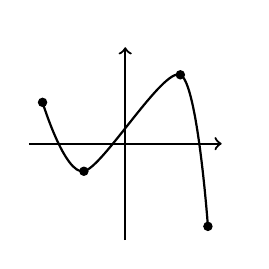
\begin{tikzpicture}[scale=.35]
                \draw[thick,->] (-3.5,0) -- (3.5,0) node[anchor=north west] {};
                \draw[thick,->] (0,-3.5) -- (0,3.5) node[anchor=south east] {};
                \draw[thick] plot[smooth] coordinates  {(-3,1.5) (-1.5,-1) (2,2.5) (3,-3)};
                \foreach \Point/\PointLabel in {(-3,1.5)/, (-1.5,-1)/, (2,2.5)/, (3,-3)/}
                \draw[fill=black] \Point circle (0.15) node[above right] {$\PointLabel$};
            \end{tikzpicture}
        \end{center}
    \end{block}
\end{frame}

\begin{frame}
    \frametitle{举例}
    对于多项式:
    $$ A(x) = x^3 + x^2 + 1 $$

    \begin{itemize}
        \item $A(x)$ 的系数为 $3$
        \item $A(x)$ 的次数界为 $4, 5, \cdots$ 等全部大于 $3$ 的数
        \item $A(x)$ 的系数表示为 $ (1, 1, 0, 1)$
        \item $A(x)$ 的一个点值表达为 $\{ (-1, 1), (0, 1), (1, 3), (2, 13) \}$
    \end{itemize}
\end{frame}

\begin{frame}
    \frametitle{表达形式的转换}
    \begin{block}{系数表达 $\Rightarrow$ 点值表达}
        直接对选取的点进行求值即可,时间复杂度为 $\textcolor{red}{\Theta(n^2)}$
    \end{block}
    \begin{block}{点值表达 $\Rightarrow$ 系数表达}
        对于给定的点值对集合 $\{ (x_0, y_0), \cdots, (x_{n-1}, y_{n-1})\}$
        使用\textbf{拉格朗日公式}
        $$A(x) = \sum_{k = 0}^{n - 1} y_k \frac{\prod_{j \neq k}(x - x_j)}{\prod_{j \neq k}(x_k - x_j)}$$
        即可求出 $A(x)$ 的系数表达。时间复杂度为 $\textcolor{red}{\Theta(n^2)}$。
    \end{block}
\end{frame}

\section{多项式的乘法}

\section{多项式的乘法}

\begin{frame}
    \frametitle{多项式的乘法}
    对于多项式乘法,如果$A(x). B(x)$均为次数界为 $n$ 的多项式,
    则它们的\textbf{乘积} $C(x)$ 是一个次数界为 $2n - 1$ 的多项式,
    对于任一属于多项式定义域的$x$,都有$C(x) = A(x)B(x)$
\end{frame}

\begin{frame}
    \frametitle{多项式的乘法}
    当多项式为\textbf{系数}表达时,其乘积的计算方法相当简单,对于表示为
    $$\vec{a} = (a_0, a_1, \cdots, a_{n-1})$$
    $$\vec{b} = (b_0, b_1, \cdots, b_{n-1})$$
    的多项式$A(x). B(x)$,其乘积$C(x)$的系数表达为:
    $$\vec{b} = (c_0, c_1, \cdots, c_{2n-1})$$
    其中
    $$c_i = \sum_{j = 0}^{i} a_j b_{i - j} \qquad \Rightarrow \textcolor{red}{\Theta(n^2)}$$
    \begin{block}{}
        $\vec{c}$ 被称为 $\vec{a}$ 和 $\vec{b}$ 的卷积,记为
        $\vec{c} = \vec{a} \otimes \vec{b}$
    \end{block}
\end{frame}

\begin{frame}
    \frametitle{多项式的乘法}
    当多项式为\textbf{点值}表达时,对于任一点$x_k$,由都有$C(x_k) = A(x_k)B(x_k)$。
    同时注意到
    $$degree(C) = degree(A) + degree(B)$$
    因此当 $A(x), B(x)$ 的点值表达分别为(注意对于$A(x),B(x)$需要$2n$个点值对)
    $$A:\{ (x_0, y_0), \cdots, (x_{2n-1}, y_{2n-1})\}$$
    $$B:\{ (x_0, y_0'), \cdots, (x_{2n-1}, y_{2n-1}')\}$$
    时,$C(x)$的点值表达应为:
    $$C:\{ (x_0, z_0), \cdots, (x_{2n-1}, z_{2n-1})\}$$
    其中
    $$z_i = y_i y_i' \qquad \Rightarrow \textcolor{green}{\Theta(n)}$$
\end{frame}


\begin{frame}
    \frametitle{多项式的乘法}
% Define a common style for blocks - this style is labeled "myBlock"
\tikzstyle{myBlock}=[draw, fill=blue!30!white, minimum size=0.5in, node distance=2.25in]

% Import TikZ library for customizing arrow heads
% i.e. an arrow head may be scaled in width/height via: -{Latex[length=2mm,width=2mm]}
\usetikzlibrary{arrows.meta}

% Define common style for path lines - this style is labeled "myPath"
\tikzstyle{myPath} = [-{Latex[length=2mm,width=2mm]}, line width=0.4mm]

\begin{figure}[H]
\centering
\begin{tikzpicture}
   \node[myBlock] (v) {\begin{tabular}{c} $\vec{a} = (a_0, a_1, \cdots, a_{n-1})$ \\ $\vec{b} = (b_0, b_1, \cdots, b_{n-1})$ \end{tabular}};
   \node[myBlock] (p) [right of=v] {$\vec{c} = (c_0, c_1, \cdots, c_{2n-1})$};
   \node[myBlock] (s) [below of=v] {\begin{tabular}{c} $A(x_0), B(x_0)$ \\ $A(x_1), B(x_1)$ \\ $\cdots$ \\ $A(x_{2n-1}), B(x_{2n-1})$ \end{tabular}};
   \node[myBlock] (b) [right of=s] {\begin{tabular}{c} $C(x_0)$ \\ $C(x_1)$ \\ $\cdots$ \\ $C(x_{2n-1})$ \end{tabular}};

   % Draw line between each of the blocks
   \draw[myPath] (v) -- (p) node [midway, above] {$\otimes$, $\textcolor{red}{\Theta(n^2)}$};
   \draw[myPath] (s) -- (b) node [midway, above] {$\times$, $\textcolor{green}{\Theta(n)}$};
   \draw[myPath] (v) -- (s) node [midway, left] {求值, $\textcolor{red}{\Theta(n^2)}$};
   \draw[myPath] (b) -- (p) node [midway, left] {插值, $\textcolor{red}{\Theta(n^2)}$};

\end{tikzpicture}
\label{fig:block_diagram}
\end{figure}

\end{frame}

\begin{frame}
    \frametitle{Can we do better?}
    使用\textbf{快速傅里叶变换},我们可以在
    $\textcolor{blue}{\Theta(n \log n)}$ 的时间复杂度下
    完成两种表示形式的转换
 
    此时我们可以在 $\textcolor{blue}{\Theta(n \log n)}$
    的时间复杂度内计算多项式的乘积
\end{frame}

\begin{frame}
    \frametitle{傅里叶变换}
    \begin{itemize}
        \item 有史以来最伟大、最深刻的发现之一
        \item 将时域信号转换为频域信号
        \item \sout{不开门课专门讲这个是计算机院学生的损失}
    \end{itemize}
    \begin{figure}
        \includegraphics[width= 0.8\linewidth]{ft.pdf}
     \end{figure}
\end{frame}

\end{document}